\documentclass[11pt,letterpaper]{article}
\usepackage[lmargin=1in,rmargin=1in,tmargin=1in,bmargin=1in]{geometry}
\usepackage{../style/homework}
\usepackage{../style/commands}
\setbool{quotetype}{true} % True: Side; False: Under
\setbool{hideans}{true} % Student: True; Instructor: False

% -------------------
% Content
% -------------------
\begin{document}

\homework{12: Due 04/14}{I was very slow in maths, geometry I actually enjoyed.}{Liam Neeson}

% Problem 1
\problem{10} Find the volume and surface area of the right circular cone shown below. [Note: Assume the line segment of length 8 below passes through the center of the circle.]
	\[
	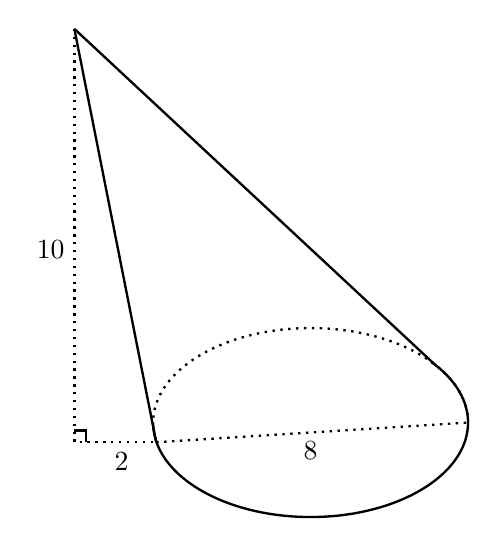
\begin{tikzpicture}
	\draw[line width=0.03cm] (-1.96,-0.25) -- (-3,5);
	\draw[line width=0.03cm] (1.58,0.735) -- (-3,5);    
	                                                           
	\draw[line width=0.03cm,dotted] (-3,5) -- (-3,-0.25) -- (-1.96,-0.25);
	\draw[line width=0.03cm] (-3,-0.1) -- (-2.85,-0.1) -- (-2.85,-0.25);
	\node at (-3.3,2.2) {$10$};
	
	\draw[line width=0.03cm,dotted] (-1.96,-0.25) -- (2,0);
	\node at (0,-0.35) {$8$};
	
	\node at (-2.4,-0.5) {$2$};
	
	\draw[line width=0.03cm,dotted] (2, 0) arc [start angle=0, end angle=180, x radius= 2, y radius= 1.2];
	\draw[line width=0.03cm] (-2, 0) arc [start angle=180, end angle=400, x radius= 2, y radius= 1.2];	
	\end{tikzpicture}
	\]



\newpage



% Problem 2
\problem{10} Find the volume and surface area of the right circular cylinder with diameter 3 and height 10 shown below.
	\[
	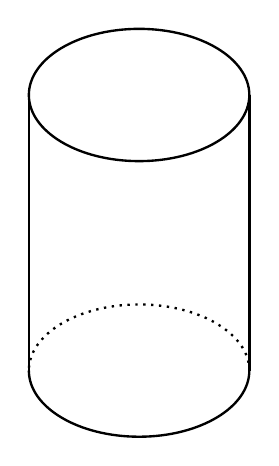
\begin{tikzpicture}[scale=0.7]
	\draw[line width=0.03cm] (0,5) ellipse (2 and 1.2);
	\draw[line width=0.03cm] (-2,5) -- (-2,0);
	\draw[line width=0.03cm] (2,5) -- (2,0);
	\draw[line width=0.03cm,dotted] (2, 0) arc [start angle=0, end angle=180, x radius= 2, y radius= 1.2];
	\draw[line width=0.03cm] (-2, 0) arc [start angle=180, end angle=360, x radius= 2, y radius= 1.2];
	\end{tikzpicture}
	\]



\newpage



% Problem 3
\problem{10} Find the volume and surface area of the cube shown below. Also, find the length of the `diagonal' of the cube, i.e. the length from one corner to another. 
 	\[
	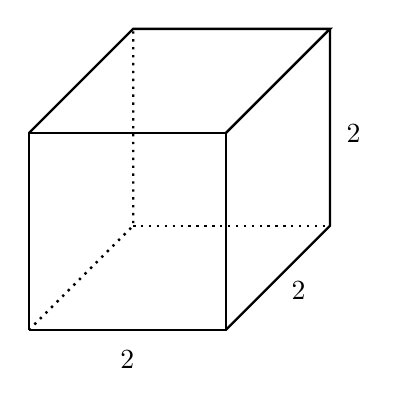
\begin{tikzpicture}[scale=2.5]
	\draw[line width=0.03cm] (0,0) -- (1,0) -- (1,1) -- (0,1) -- (0,0);
	\draw[line width=0.03cm] (0,1) -- (0.53,1.53) -- (1.53,1.53) -- (1,1);
	\draw[line width=0.03cm] (1.53,1.53) -- (1.53,0.53) -- (1,0);
	\draw[line width=0.03cm, dotted] (0,0) -- (0.53,0.53) -- (0.53,1.53);
	\draw[line width=0.03cm, dotted] (0.53,0.53) -- (1.53,0.53);
	\node at (0.5,-0.15) {$2$};
	\node at (1.37,0.2) {$2$};
	\node at (1.65,1) {$2$};
	\end{tikzpicture}
	\]


\end{document}